\section{Versuchsdurchführung}
\subsection{Federpendel}
Bei diesem ersten Versuchsteil sollte die Federkonstante $D$ der Feder eines Federpendels auf zwei Arten bestimmt werden. Die erste Methode war die statische Bestimmung, bei welcher die Auslenkung der Feder $x$ aus der Ruhelage $x_0$ bei drei verschiedenen Gewichtsstücken $m$ die Grundlage der Berechnungen war. Hierzu wurde zuerst die Position der Waagschale in Ruhelage, also ohne zusätzliche Gewichtsstücke, gemessen. Danach wurden die Massestücke nacheinander auf die Waagschale gelegt und jeweils die resultierende Position erfasst. Als zweite Methode diente die dynamische Bestimmung, bei der $D$ über die Masse und die Schwingungsdauer bestimmt wurde. Gemessen wurde hierbei die Dauer für 50 Schwingungen $t_{50}$ um Messunsicherheiten zu verringern. Die Differenz zur Ruheposition ergab die Auslenkung. Zuletzt wurden noch die Masse der Waagschale und der Feder bestimmt, da diese ebenfalls für die dynamische Berechnung benötigt werden.
\subsection{Fadenpendel}
Im zweiten Versuchsteil sollte die Erdbeschleunigung $g$ durch die Schwingungsdauer eines Fadenpendels bestimmt werden. Hierzu wurde das Pendel bei drei verschiedenen Längen $l$ um einen kleinen Winkel ausgelenkt und die benötigte Zeit für 50 Schwingungen gestoppt. Die Länge des Pendels wurde durch die Addition des Radius der Kugel und der Länge der Pendelschnur bestimmt.
\subsection{gekoppeltes Pendel}
Beim gekoppelten Pendel war die Aufgabe, den Kopplungsgrad $k$ und die relative Frequenzaufspaltung $\frac{\Delta \omega}{\omega_0}$ für 2 verschieden harte Federn (Kupfer und Eisen) zu bestimmen. Die Aufhängung der Feder wurde vorab auf einer Ebene ca. im zweiten Drittel der gesamten Pendellänge festgesetzt. Zudem wurde sichergestellt, dass die Schwingungsdauern beider Pendel übereinstimmten. 
\subsubsection{statische Bestimmung des Kopplungsgrades}
Die erste Art der Bestimmung von $k$ war die statische Bestimmung über die Auslenkung der Pendel. Hierzu wurde ein Pendel um $x_1=\SI{10,0+-0,2}{cm}$ von der Ruheposition ausgelenkt. Dies resultierte in folgenden Auslenkungen des gekoppelten Pendels:\\
\textbf{Kupferfeder}
$x_2=\SI{1,2+-0,4}{cm}$\\
\textbf{Eisenfeder}
$x_2=\SI{2,1+-0,4}{cm}$
\subsubsection{dynamische Bestimmung des Kopplungsgrades}
\label{durchgekop}
Nach einer kurzen Einführung durch den Versuchsbetreuer in den Umgang mit dem Ultraschall-Entfernungssensor wurde die Schwingungsdauer $T_0=\SI{2,48+-0,02}{s}$ eines einzelnen Pendels durch Stoppen der Dauer für 50 Schwingungen bestimmt. Dann wurde das Doppelpendel für jede Feder jeweils zu einer gleichsinnigen und gegensinnigen Schwingung angeregt. Mithilfe des Ultraschall-Entfernungssensors wurde die Schwingung aufgezeichnet. Die Periodendauer $T_{gl}$ und $T_{geg}$ konnte nun aus der vom Messprogramm berechneten Frequenz $f_{gl}$ und $f_{geg}$ berechnet werden.\footnote{Werte siehe Laborbuch} Während des Versuchs wurde von uns festgestellt, dass es schwierig war eine gleichsinnige Schwingung in Gang zu bringen, da dort Schwebungen auftraten, sodass wir mehrere Versuche benötigten um diese Schwebungen gering zu halten. Bei den gegensinnigen Schwingungen trat dieses Problem nur in einem viel geringeren Maß auf.

Als nächstes wurde das System zu Schwebungen angeregt indem ein Pendel ausgelenkt wurde, während das andere auf der Ruhelage festgehalten wurde. Wenn nun beide Pendel gleichzeitig losgelassen wurden konnten zuverlässig Schwebungen produziert werden. Jedoch war es auch hier schwierig, eine perfekte Schwebung zu erzeugen (siehe auch z.B. \cref{fig:schwebung-Bwg-Cu}). Bei diesem Teil des Experiments traten zusätzlich massive Fehler mit dem Messprogramm auf. Zu den in \cref{messgekop} erwähnten Problemen funktionierte zusätzlich die Berechnung der Frequenzen nicht mehr zuverlässig. Während bei der Eisenfeder keine Probleme auftauchten und das Programm zwei Peaks im Frequenzverlauf anzeigte welche auch mit $f_{gl}$ und $f_{geg}$ übereinstimmten, wurde uns bei der Auswertung der Kupferfeder zuerst nur ein Peak angezeigt. Auch mithilfe des Versuchsbetreuers und nach mehrmaligem erneuten Messen mit verschiedenen Abtastraten des Entfernungmessers konnte kein reproduzierbarer Frequenzverlauf erzeugt werden. Die beste Messung mit zwei Peaks (\cref{fig:schwebung-Bwg-Cu-FFT})
zeigte eine ungefähre Übereinstimmung mit $f_{gl}$, der zweite Peak ist aber weit abseits des Wertes von $f_{geg}$. 

\section{Versuchsauswertung- und Ergebnisse}
\subsection{Federpendel}
Bei der statischen Berechnung betrachten wir nur Massen- und Auslenkungsdifferenzen, weshalb hier bei der Rechnung nur die jeweils anghängten Massestücke als Gewicht in die Rechnung eingehen (Die Masse der Waagschale und Feder ist hier also nicht von Bedeutung). Aus den gemessenen Werten und \cref{eq1.1} ergibt sich für die statische Bestimmung der Federkonstante $D=\SI{12520,5+-1954,29}{g/s^2}$.
Bei der dynamischen Bestimmung der Federkonstante ergibt sich der Wert $D=\SI{12836+-17,94}{g/s^2}$. Hierbei wurden die in der Rechnung verwendeten Massen durch Addition des Gewichts der jeweiligen Massestücke, der Waagschale und einem Drittel der Masse des Pendels berechnet.
\subsection{Fadenpendel}

\subsection{gekoppeltes Pendel}
Bei der Eisenfeder passten die Werte der einzelnen Bestimmung von $f_{gl}=\SI{0,430+-0,001}{Hz}$ und $f_{geg}=\SI{0,590+-0,001}{Hz}$ genau zu den Werten der Schwebung. Da die Messung der Kupferfeder wie in \cref{durchgekop} beschrieben nicht zuverlässig durchführbar war, ist es keine Überraschung, dass auch die Werte der Schwebung von $f_{gl}$ eine  Abweichung von $\SI{0,02+-0,002}{Hz}$ vom Wert der Einzelbestimmung aufzeigt.
\subsubsection{statische Bestimmung des Kopplungsgrades}
\textbf{Kupferfeder}
$x_1=\SI{10,0+-0,2}{cm}$ und $x_2=\SI{1,2+-0,4}{cm}$ also ist $k=\frac{x_2}{x_1}=\SI{0,12+-0,02}{}$\\
\textbf{Eisenfeder}
$x_1=\SI{10,0+-0,2}{cm}$ und $x_2=\SI{2,1+-0,4}{cm}$ also ist $k=\frac{x_2}{x_1}=\SI{0,21+-0,02}{}$
\subsubsection{dynamische Bestimmung des Kopplungsgrades}
Aus den Periodendauern lässt sich mit \cref{eq1.12} der Kopplungsgrad bestimmen.

\textbf{Kupferfeder}\\
$T_{gl}=\SI{2,439+-0,006}{s}$ und $T_{geg}=\SI{1,960+-0,004}{s} \Rightarrow k=\SI{21,52+-0,06e-2}{}$

\textbf{Eisenfeder}\\
$T_{gl}=\SI{2,326+-0,005}{s}$ und $T_{geg}=\SI{1,695+-0,003}{s}\Rightarrow k=\SI{30,63+-0,07e-2}{}$\\
\subsubsection{Bestimmung der relativen Frequenzaufspaltung}
Die relative Frequenzaufspaltung $\frac{\Delta \omega}{\omega_0}$ ist mit $k$ aus der statischen Bestimmung und \cref{eq1.13} \\ $\frac{\Delta \omega}{\omega_0}=0,1282\pm 0,0229$ für die Kupferfeder und \\ $\frac{\Delta \omega}{\omega_0}=0,2376\pm 0,0259$ für die Eisenfeder.

Mit \cref{eq1.14} ergeben sich hingegen folgende Werte:\\
$\frac{\Delta \omega}{\omega_0}=0,1281 \pm 0,0228$ für die Kupferfeder und\\
$\frac{\Delta \omega}{\omega_0}=0,2367 \pm 0,0255 $ für die Eisenfeder.

Die benutze Näherung ist also offensichtlich sowohl beim Funktionswert als auch beim Fehlerwert bis auf die dritte Nachkommastelle genau.
\subsection{Doppelpendel}

Bei großen Winkeln verhält sich das Doppelpendel chaotisch, also ohne irgendein erkennbares Muster. Dies lässt sich dadurch erklären, dass die Bewegungsgleichungen keine lineare Differentialgleichungen sind und sich das System somit auch nicht wie ein harmonischer Oszillator verhält. Bei kleineren Auslenkungen beruhigt sich dieses Verhalten und es ist eine klare Periodizität erkennbar. Nun wirkt die Kleinwinkelnäherung und die Differentialgleichungen werden linear.
\clearpage

\section{Graphische Darstellung der Ergebnisse}
%Text dazu, dass gespeicherte MEssergebnisse anders sind als vor Ort.
Die wirklich abgelesene Frequenz in der Fouriertransformation wird durch einen Punkt angezeigt

\subsection{Kopplung durch Cu-Feder}

\begin{figure}[h!]
\centering
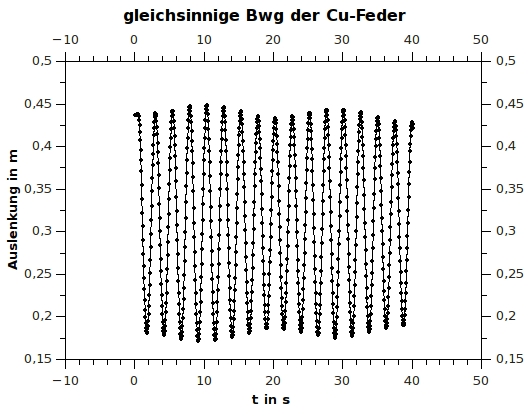
\includegraphics[width=0.6\linewidth]{../Messungen/graphen/gleich-Bwg-Cu}
\caption{Beide Pendel schwingen möglichst gleichphasig}
\label{fig:gleich-Bwg-Cu}
\end{figure}

\begin{figure}[h!]
\centering
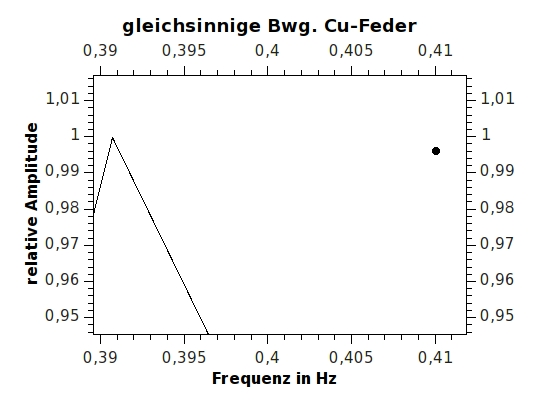
\includegraphics[width=0.55\linewidth]{../Messungen/graphen/gleich-Bwg-Cu-FFT}
\caption{Die dazugehörige Fouriertransformation}
\label{fig:gleich-Bwg-Cu-FFT}
\end{figure}

\clearpage

\begin{figure}[h!]
\centering
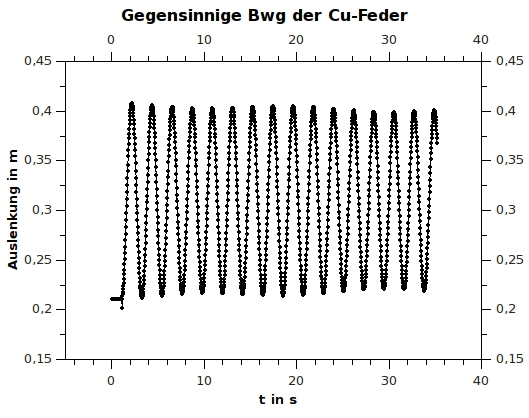
\includegraphics[width=0.55\linewidth]{../Messungen/graphen/gg-Bwg-Cu}
\caption{Beide Pendel schwingen möglichst gegenphasig}
\label{fig:gg-Bwg-Cu}
\end{figure}

\begin{figure}[h!]
\centering
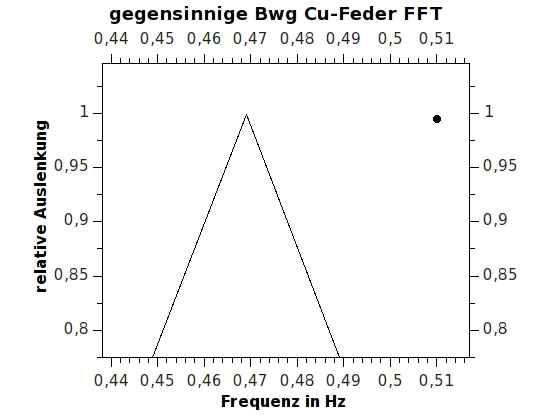
\includegraphics[width=0.7\linewidth]{../Messungen/graphen/gg-Bwg-Cu-FFT}
\caption{Die dazugehörige Fouriertransformation}
\label{fig:gg-Bwg-Cu-FFT}
\end{figure}

\clearpage
\begin{figure}[h!]
\centering
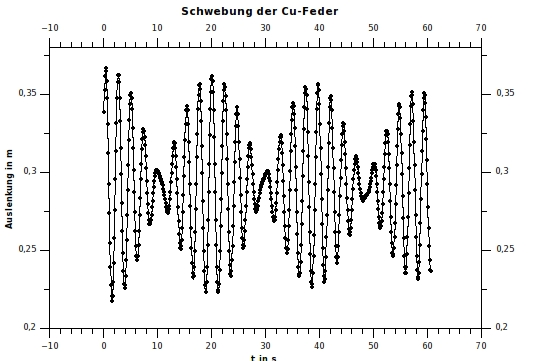
\includegraphics[width=0.7\linewidth]{../Messungen/graphen/schwebung-Bwg-Cu}
\caption{Die Pendel werden zu Schwebungen angeregt}
\label{fig:schwebung-Bwg-Cu}
\end{figure}

\begin{figure}[h!]
\centering
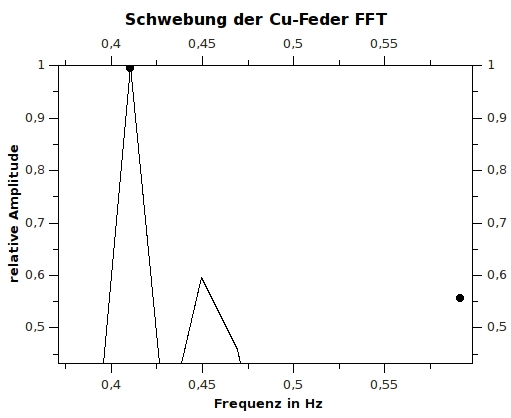
\includegraphics[width=0.7\linewidth]{../Messungen/graphen/schwebung-Bwg-Cu-FFT}
\caption{Die dazugehörige Fouriertransformation}
\label{fig:schwebung-Bwg-Cu-FFT}
\end{figure}

\clearpage

\subsection{Kopplung durch Fe-Feder}

\begin{figure}[h!]
\centering
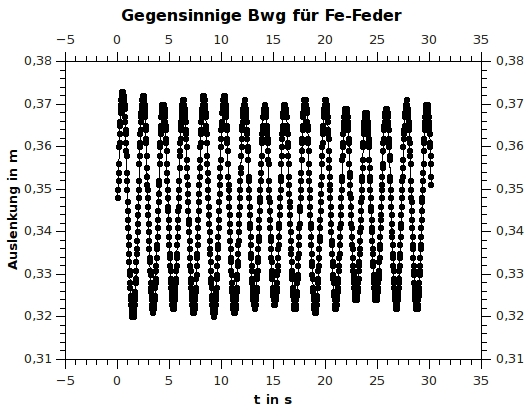
\includegraphics[width=0.65\linewidth]{../Messungen/graphen/gg-Bwg-Fe}
\caption{Die Pendel schwingen möglichst gegenphasig}
\label{fig:gg-Bwg-Fe}
\end{figure}

\begin{figure}[h!]
\centering
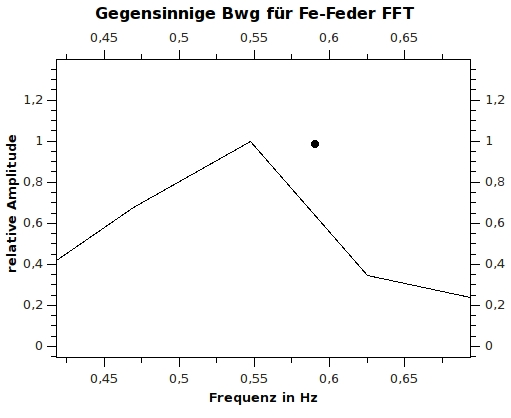
\includegraphics[width=0.7\linewidth]{../Messungen/graphen/gg-Bwg-Fe-FFT}
\caption{Die dazugehörige Fouriertransformation}
\label{fig:gg-Bwg-Fe-FFT}
\end{figure}

\clearpage

\begin{figure}[h!]
\centering
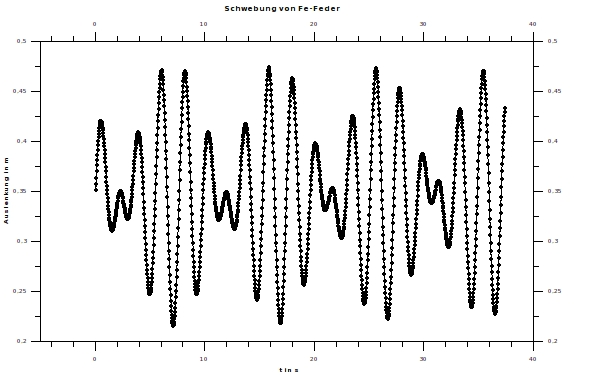
\includegraphics[width=0.7\linewidth]{../Messungen/graphen/schwebung-Fe}
\caption{Die Pendel wurden zu Schwebungen angeregt}
\label{fig:schwebung-Fe}
\end{figure}

\begin{figure}[h!]
\centering
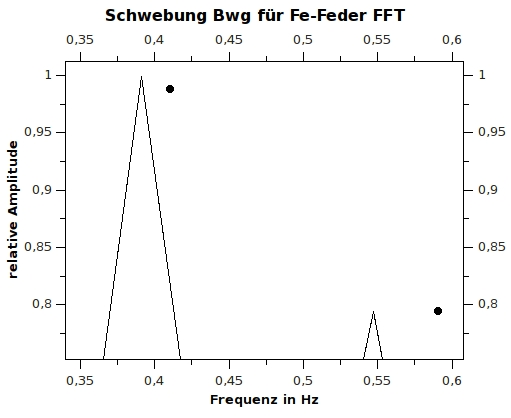
\includegraphics[width=0.7\linewidth]{../Messungen/graphen/SchwebungvonFe-FederFFT}
\caption{Die dazugehörige Fouriertransformation}
\label{fig:SchwebungvonFe-FederFFT}
\end{figure}

\clearpage

\section{Einordnung der Ergebnisse, Literaturvergleich und Diskussion}

Beim ersten Teilversuch stimmen die Ergebnisse im Fehlerbereich überein. Bei den Messungen und der Auswertung sind keine groben Fehler passiert. Man erkennt an der Größenordnung der Fehler, dass die statische Methode deutlich ungenauer ist als die dynamische Methode. Bei ersterem ist die statische Auslenkung aufgrund von kleinen Schwingungen nur ungenau zu bestimmen. Bei Letzterem musste nur die Periodendauer gemessen werden, was genau durchführbar ist, wenn man die Zeit für 50 Perioden misst.

Bei der Bestimmung der Erdbeschleunigung stimmt unsere Messung mit dem Literaturwert im Fehlerbereich überein. Jedoch ist dieser Fehler mit über 10\% recht groß, was auf die Vereinfachungen zurückzuführen ist. So wurde der Faden als masselos aufgefasst sowie die reale Ausdehnung der Kugel ebenso wie die Reibung vernachlässigt. Die Messung der Fadenlänge war mit dem Maßband ebenfalls ungenau.

Die Kopplungsgrade bei beiden Kopplungen stimmen nicht im Fehlerbereich überein. Die Ursache liegt in der fehlenden Kalibrierung des Ultraschallsensors sowie dem fehlerhaften Programm mit dem die Auswertung geschah. %ref müssen rein

\section{Physikalische Interpretation}

Die Messung der Erdbeschleunigung ist mit dem Fadenpendel nicht genau möglich. Es müssen zu viele Annahmen gemacht werden, als dass der reale Wert genau ermittelt werden könnte. Mit einem Federpendel (mit bekannter Federhärte) hingegen wäre die Messung viel genauer, da keine Annahmen gemacht werden müssen. Die Messfehler können durch Messung von mehreren Schwingungsperioden minimiert werden, so dass ein genauerer Wert für die Erdbeschleunigung als beim Fadenpendel bestimmt werden kann.
